% -*- latex -*-
%%%%%%%%%%%%%%%%%%%%%%%%%%%%%%%%%%%%%%%%%%%%%%%%%%%%%%%%%%%%%%%%
%%%%
%%%% This TeX file is part of the course
%%%% Scientific Computing in C++23
%%%% copyright 2023-2024 Victor Eijkhout eijkhout@tacc.utexas.edu
%%%%
%%%% d2dtests.tex : test results
%%%%
%%%%%%%%%%%%%%%%%%%%%%%%%%%%%%%%%%%%%%%%%%%%%%%%%%%%%%%%%%%%%%%%

\Level 0 {Introduction}

In this paper we consider the parallelization of the `power method'.

%%packtsnippet d2dpower
Computationally, the power method is an attractive paradigmatic example
in that it exhibits the most common parallelism patterns:
\begin{itemize}
\item independent or `convenient' parallelism;
\item global reduction operations
\item point-to-point communications.
\end{itemize}
As follows.
The method is given by
\begin{quote}
  \begin{tabbing}
    Let $A$ a matrix of interest\\
    Let $x$ be a random vector\\
    For \=iterations until convergence\\
    \> compute the product $y\leftarrow Ax$\\
    \> compute the norm $\gamma=\| y \|$\\
    \> normalize $x\leftarrow y/\gamma$\\
  \end{tabbing}
\end{quote}
where in the limit $\gamma$ will be the
largest eigenvalue of~$A$,
and $x$ the corresponding eigenvector.

The basis to parallelizing the power method lies in the distribution of~$x$.
Each processing element~$p$, whether that be a core or processor,
takes care (in a sense that we will later defined)
of a disjoint set of indices~$I_p$.
The operations then are:
\begin{itemize}
\item The normalization step has independent parallelism:
  each component $y_i=x_i/\gamma$ can be independently computed,
  so each process~$p$ can compute $y_i$ for~$i\in I_p$ fully independently;
\item Computing $\gamma$ is a all-reduction:
  each processing element $p$ first computes $\gamma_p=\sqrt{\sum_{i\in I_p}y_i^2}$
  independently,
  and $\gamma=\sqrt{\sum_p\gamma_p}$ is then formed by combination, and
  made available to all~$p$;
\item Finally, for the operator $A$ we assume a sparse matrix,
  for instance a \acf{FD} stencil for a \ac{PDE}, or a \indexterm{convolution} kernel.
  This is characterized by each component $y_i$ of the output needing several
  components $x_j$ of the input.
\end{itemize}
%%packtsnippet end

\Level 1 {Loop parallelism in our example}
%%packtsnippet d2dloops
\label{sec:d2d-omp1d}

In our power method application
%% (chapter~\ref{ch:parexample})
a first example of a parallel loop is scaling an array by a factor.
%
\cxxverbatimsnippet{d2dscaleoned}

Some remarks.
\begin{enumerate}
\item
  The loop bounds are set to range only over the size of the interior
  of the \lstinline{mdspan}.
  Later we will explore using a range-based loop and
  dispensing with indexing entirely.
  However, that is not always possible.
\item We are using a tradition macro to translate from two-dimensional
  to one-dimensional indexing, skipping the border points:
  \cxxverbatimsnippet{d2donedindex}
  Later we will discuss other indexing schemes.
\begin{packt}
    (For the macro idiom, see section~\ref{sec:cpp-mac-param}.)
\end{packt}
\item
  The \lstinline{data2d} method gives an \lstinline{mdspan} object:
  
  \twosnippetswithcaptions{Class data:}{d2dspan0}{Accessor:}{d2dspan2}

  so we can use the two-dimensional \lstinline{[i,j]} type indexing.
\end{enumerate}

%%packtsnippet end

\Level 1 {Reduction in the example application}
%%packtsnippet d2dreduction

The $\ell_2$ reduction of our example application
looks in code like:
%
\cxxverbatimsnippet{d2dnormspan}

\begin{figure}[t]
  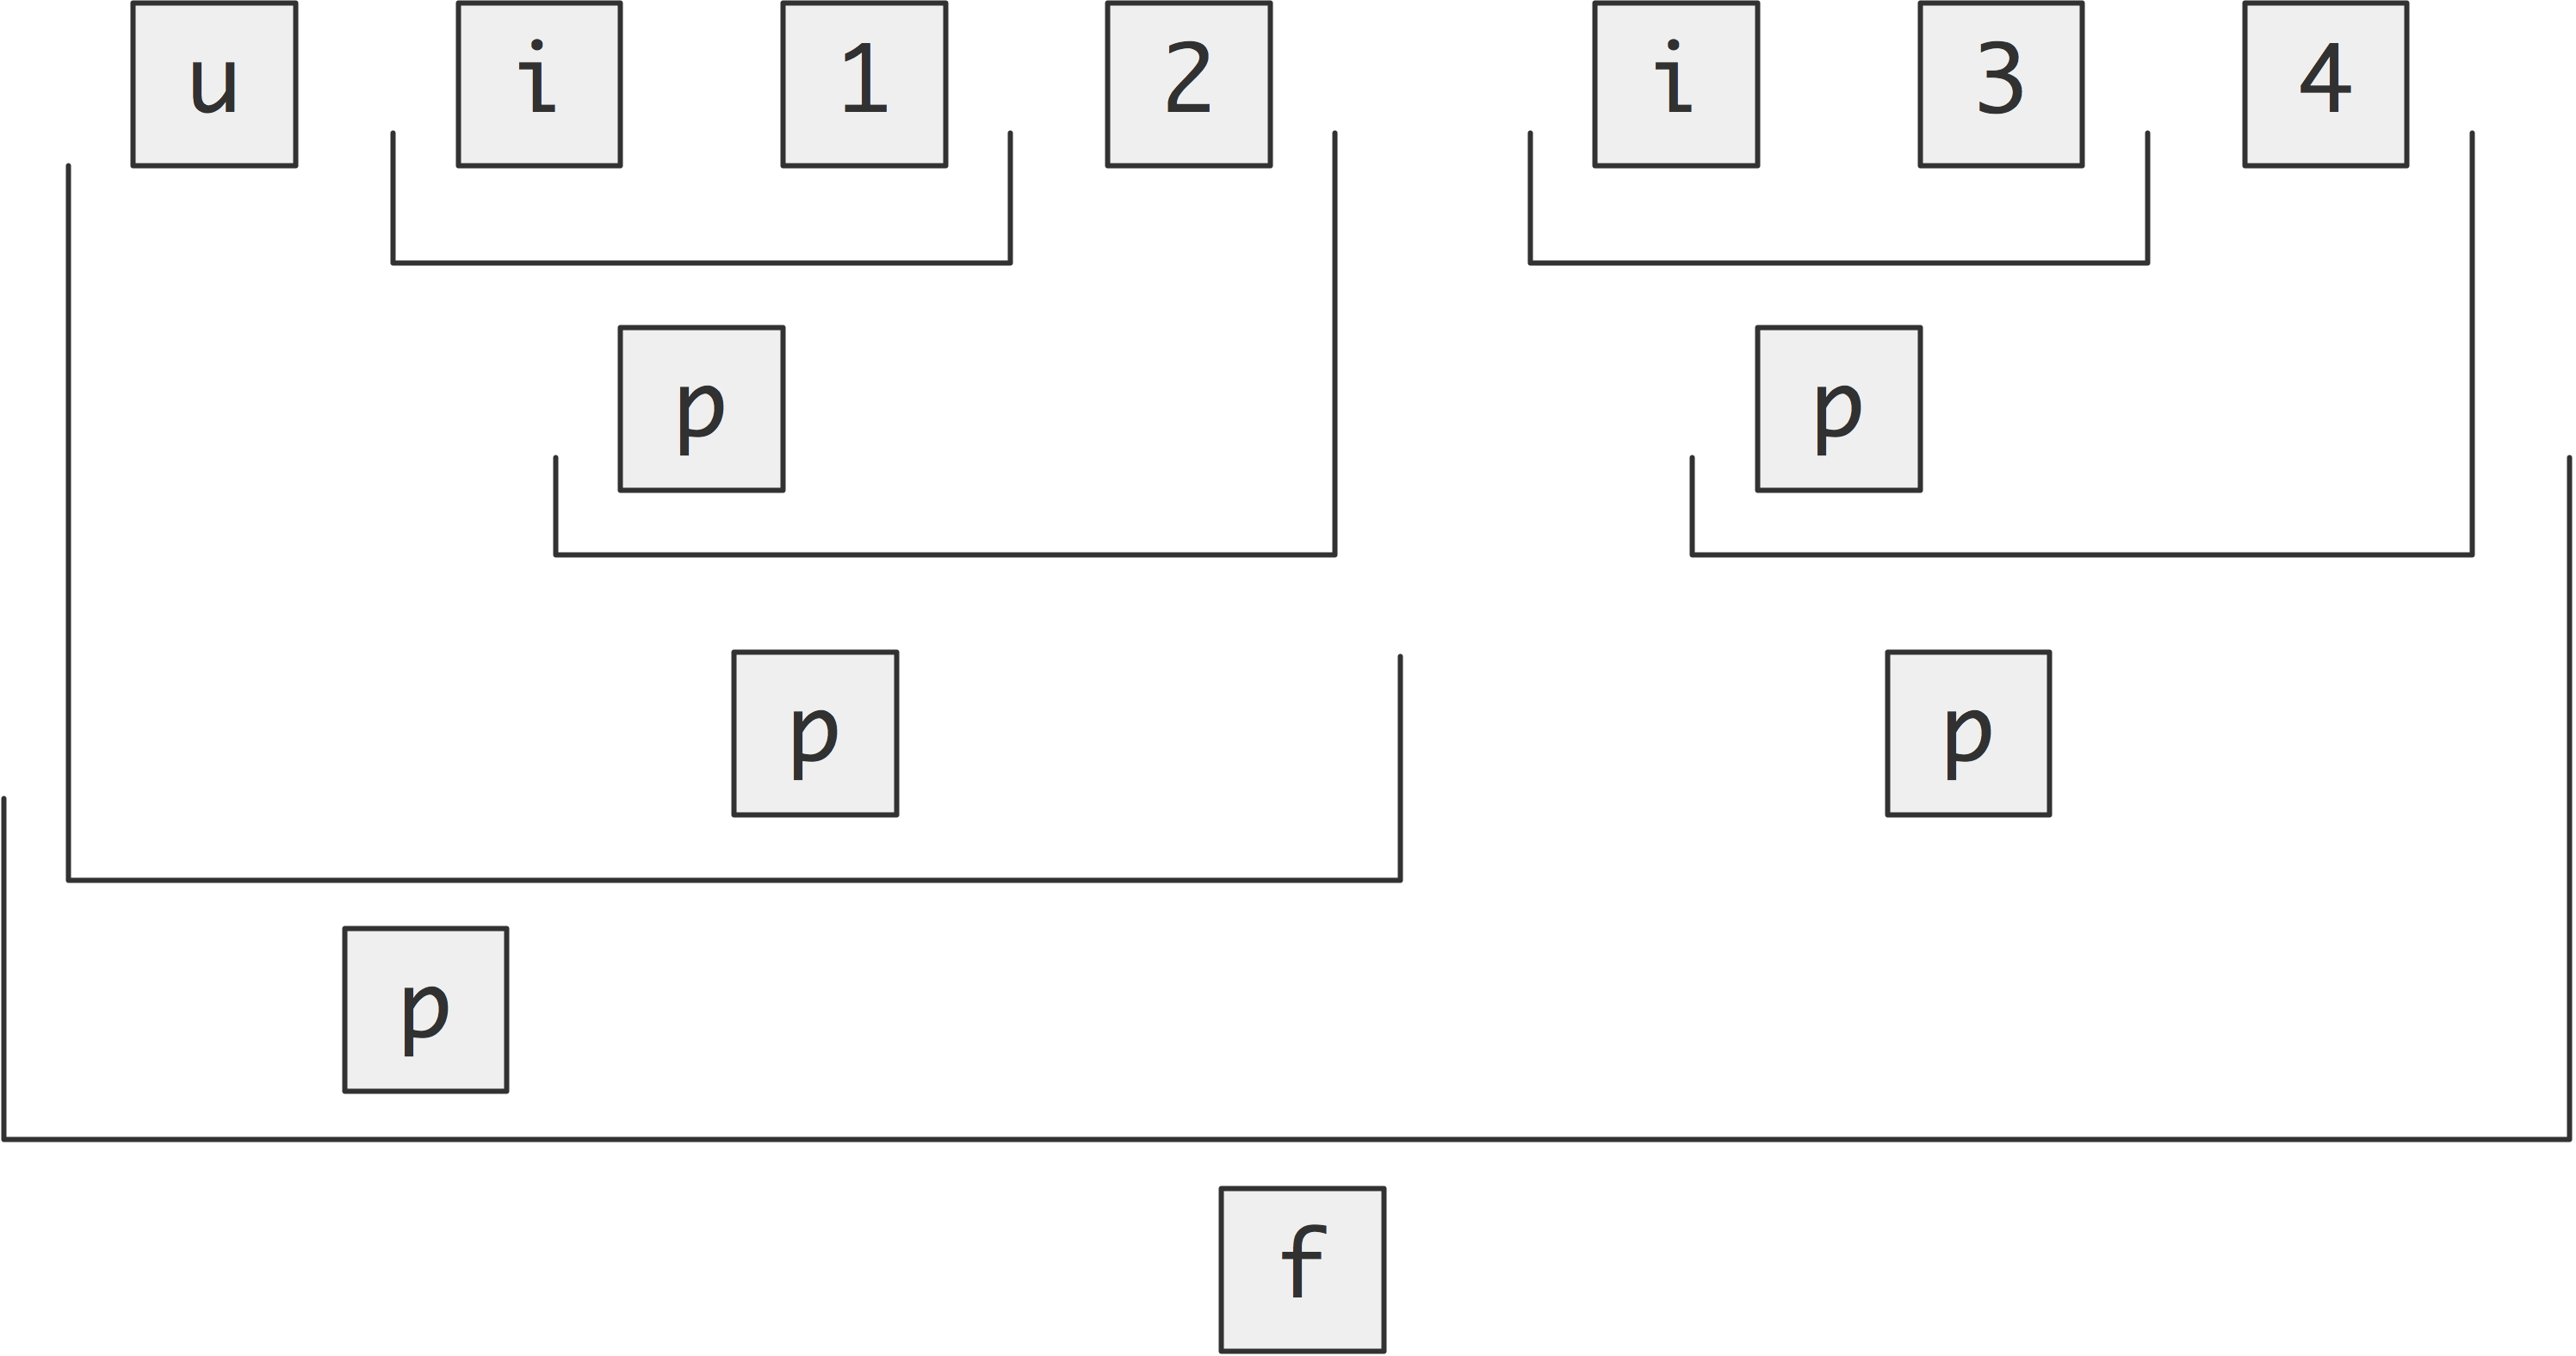
\includegraphics[scale=.1]{omp-reduct}
  \caption{Structure of a reduction of four items on two threads,
    where $u$ is the user-supplied initial value,
    and $i$~is the natural initial value for the reduction operator.}
  \label{fig:omp-reduct}
\end{figure}

OpenMP resolves the race condition on the reduction variable
by giving each thread a local copy of \lstinline{sum_of_squares},
summing into that, and adding the local copies together in the end.

%%packtsnippet end

\Level 1 {Five-point stencil}
%%packtsnippet d2d5pt
\label{sec:d2d-5pt}

The evaluation of the 5-point difference operator is perfectly parallel
in that there are no dependencies between the points of the output vector.
However, the loop is more complicated than the scaling operation above:
%
\cxxverbatimsnippet{d2d5ptoned}

While this operation is somewhat like a `transform' range operation,
the complexity of the right-hand-side indexing precludes using
an actual range algorithm.
Therefore, in later versions of this code we will range over
the indices, rather than the actual data.

%%packtsnippet end

\Level 0 {Example application: tests and discussion}

There are various ways we can parallelize our example application.

\Level 1 {Indexing mode 1D}

Above in section~\ref{sec:d2d-omp1d}
we already showed the simplest parallelization scheme:
we loop two-dimensionally over the index space,
and translate that through a \ac{CPP} macro
to one-dimensional indexing in a traditional container.
The loops are then parallelized by OpenMP.

In graphs to follow we indicate this mode by~\n{oned}.

We designate by \n{clps} this same code, but adding
\lstinline{collapse(2)} to each OpenMP loop nest.

\Level 1 {\texttt{mdspan} indexing}

While the scaling and the norm calculation can be expressed as range algorithms,
doing so for the five-point stencil update is trickier,
so we take a two-step approach:
\begin{enumerate}
\item We access data through an \lstinline{mdspan}, so that have multidimensional indexing:

  \twosnippets{d2dspan0}{d2dspan2}

\item We define the iteration space as a \indexc{cartesian_product} range view:

  \cxxverbatimsnippet{d2dinner}

\end{enumerate}
This allows us to write, cleanly and compactly:
\cxxverbatimsnippet{d2d5ptspan}

In graphs to follow we indicate this mode by~\n{span}.

\Level 1 {DIY cartesian product}

The \lstinline{cartesian_product} view is quite general
so one could wonder about overhead.
We write a custom iterator over a contiguous domain.
It maintains internally \lstinline{i,j} coordinates
which are updated as follows:
%
\cxxverbatimsnippet{d2ddiyiter}

\Level 1 {Kokkos and Sycl}

We also use the Kokkos and Sycl libraries in their `host' mode.
In graphs to follow we indicate these modes
by \n{kokkos} and \n{sycl} respectively.

\Level 2 {Sycl}

Sycl is an open standard that targets
heterogeneous parallelism through strict standard C++.

The preferred mechanism for handling memory coherence is through buffers.
Host memory is wrapped in a buffer structure:
\cxxverbatimsnippet{syclbufcreate}

This memory can then transparently be accessed in a kernel, where
coherence is ensured by the runtime.
This turns out to be as efficient as more explicit mechanisms.
%
\cxxverbatimsnippet{syclbufaccess}
%
Note that Sycl has a true two-dimensional indexing mode.

We see that the \lstinline{parallel_for} construct
resembles a C++ range algorithm: it combines
a range --~though of the index space, not the data space~--
and a lambda expression to be applied at each point.

Note the, somewhat contrived, index shifting that we have to apply
in order to range over the interior of the index space.

\Level 2 {Kokkos}

Kokkos is the execution layer of the Trilinos project.
It is, like Sycl, a data-parallel programming mode
that supports by host and device execution with the same code.
Unlike Sycl there is no explicit queue; instead,
objects are explicitly associated with the host or device data space.

\cxxverbatimsnippet{kokkosbufcreate}

Like Sycl, there are explicit parallelism constructs.
These closely resemble C++ range algorithms,
specifying an explicit index space over which to iterate,
and the lambda expression to apply at each index.

\cxxverbatimsnippet{kokkosbufaccess}

\Level 1 {Timing comparison}

Let's compare various implementation strategies.
Test given here are on an \indextermbus{Intel}{Sapphire Rapids}
dual socket node with 112 cores total.
We compare the Intel~2024 (figure~\ref{fig:diff2d-variants-intel})
and GCC~13 (figure~\ref{fig:diff2d-variants-gcc})
compilers.

\begin{figure}[t]
  \pgfplotsset{table/col sep=comma}
  \begingroup %\begin{multicols}{2}
    \tikzsetnextfilename{diff2d-ratios-intel-spr}
    \begin{tikzpicture}
      \begin{semilogyaxis}[
          title=Execution time,
          ylabel=time, xlabel=cores,
          width=.5\textwidth, height=.5\textwidth,
          legend entries={oned,clps,span,iota,kokkos,sycl,},
          legend pos=north east,
        ]
        \addplot table[y=oned]{plots/spr-ratios-intel.csv};
        \addplot table[y=clps]{plots/spr-ratios-intel.csv};
        \addplot table[y=span]{plots/spr-ratios-intel.csv};
        \addplot table[y=iota]{plots/spr-ratios-intel.csv};
        \addplot table[y=kokkos]{plots/spr-ratios-intel.csv};
        \addplot table[y=sycl]{plots/spr-ratios-intel.csv};
      \end{semilogyaxis}
    \end{tikzpicture}
    %\columnbreak
    \tikzsetnextfilename{diff2d-ratios-intel-spr-sp}
    \begin{tikzpicture}
      \begin{axis}[
          title=Ratio to oned,
          ylabel=ratio, ymax=20, xlabel=cores,
          width=.5\textwidth, height=.5\textwidth,
          legend entries={oned,clps,span,iota,kokkos,sycl,},
          legend pos=north west,
        ]
        \addplot table[y=oned]{plots/spr-ratios-intel-rat.csv};
        \addplot table[y=clps]{plots/spr-ratios-intel-rat.csv};
        \addplot table[y=span]{plots/spr-ratios-intel-rat.csv};
        \addplot table[y=iota]{plots/spr-ratios-intel-rat.csv};
        \addplot table[y=kokkos]{plots/spr-ratios-intel-rat.csv};
        \addplot table[y=sycl]{plots/spr-ratios-intel-rat.csv};
      \end{axis}
    \end{tikzpicture}
  \endgroup %\end{multicols}
  \caption{Comparing implementation strategies, Intel 2024 compiler on a 112-core Sapphire Rapids node.}
  \label{fig:diff2d-variants-intel}
\end{figure}

\begin{figure}[t]
  \pgfplotsset{table/col sep=comma}
  \begingroup %\begin{multicols}{2}
    \tikzsetnextfilename{diff2d-ratios-gcc-spr}
    \begin{tikzpicture}
      \begin{semilogyaxis}[
          title=Execution time,
          ylabel=time, xlabel=cores,
          width=.5\textwidth, height=.5\textwidth,
          legend entries={oned,clps,span,diy2d,kokkos,},
          legend pos=north east,
        ]
        \addplot table[y=oned]{plots/spr-ratios-gcc.csv};
        \addplot table[y=clps]{plots/spr-ratios-gcc.csv};
        \addplot table[y=span]{plots/spr-ratios-gcc.csv};
        \addplot table[y=diy2d]{plots/spr-ratios-gcc.csv};
        \addplot table[y=kokkos]{plots/spr-ratios-gcc.csv};
      \end{semilogyaxis}
    \end{tikzpicture}
    %\columnbreak
    \tikzsetnextfilename{diff2d-ratios-gcc-spr-sp}
    \begin{tikzpicture}
      \begin{axis}[
          title=Ratio to oned,
          ylabel=ratio, ymax=12, xlabel=cores,
          width=.5\textwidth, height=.5\textwidth,
          legend entries={oned,clps,span,diy2d,kokkos,},
          legend pos=north west,
        ]
        \addplot table[y=oned]{plots/spr-ratios-gcc-rat.csv};
        \addplot table[y=clps]{plots/spr-ratios-gcc-rat.csv};
        \addplot table[y=span]{plots/spr-ratios-gcc-rat.csv};
        \addplot table[y=diy2d]{plots/spr-ratios-gcc-rat.csv};
        \addplot table[y=kokkos]{plots/spr-ratios-gcc-rat.csv};
      \end{axis}
    \end{tikzpicture}
  \endgroup %\end{multicols}
  \caption{Comparing implementation strategies, Gcc 2024 compiler on a 112-core Sapphire Rapids node.}
  \label{fig:diff2d-variants-gcc}
\end{figure}

\begin{figure}[t]
  %% diff2d-scaling-span-skx-intel-20000.csv diff2d-scaling-span-skx-intel-20000-sp.csv
  \pgfplotsset{table/col sep=comma}
  \hbox\bgroup %%\begin{multicols}{2}
    \tikzsetnextfilename{diff2d-procs}
    \begin{tikzpicture}
      \begin{semilogyaxis}[
          title=Runtime,
          ylabel=msec, xlabel=cores,
          width=.55\textwidth, height=.5\textwidth,
          legend entries={skx,icx,spr,grx},
        ]
        \addplot table[y=skx]{plots/intel-oned-skx-32000.csv};
        %%\addplot table[y=csx]{plots/intel-oned-csx-32000.csv};
        \addplot table[y=icx]{plots/intel-oned-icx-32000.csv};
        \addplot table[y=spr]{plots/intel-oned-spr-32000.csv};
        \addplot table[y=grx]{plots/intel-oned-grx-32000.csv};
      \end{semilogyaxis}
    \end{tikzpicture}
    %% \columnbreak
    \tikzsetnextfilename{diff2d-procs-bw}
    \begin{tikzpicture}
      \begin{axis}[
          title=Speedup,
          ylabel=$S_p$, xlabel=cores,
          width=.55\textwidth, height=.5\textwidth,
          legend entries={skx,icx,spr,grx},
          legend pos=north west,
        ]
        \addplot table[y=skx]{plots/intel-oned-skx-32000-sp.csv};
        %%\addplot table[y=csx]{plots/intel-oned-csx-32000-sp.csv};
        \addplot table[y=icx]{plots/intel-oned-icx-32000-sp.csv};
        \addplot table[y=spr]{plots/intel-oned-spr-32000-sp.csv};
        \addplot table[y=grx]{plots/intel-oned-grx-32000-sp.csv};
      \end{axis}
    \end{tikzpicture}
  \egroup %%\end{multicols}
  \caption{Generations of Intel processors (OpenMP)}
  \label{fig:diff2d-procs}
\end{figure}

In figure~\ref{fig:diff2d-procs} we compare three generations of Intel processors:
\begin{itemize}
\item \indextermbus{Intel}{Sky Lake} in the \indextermbus{TACC}{Stampede2} cluster,
  in a two-socket configuration with a total of 40 cores;
\item \indextermbus{Intel}{Cascade Lake} in the \indextermbus{TACC}{Frontera} cluster,
  in a two-socket configuration with a total of 56 cores;
\item \indextermbus{Intel}{Ice Lake} in the \indextermbus{TACC}{Stampede3} cluster,
  in a two-socket configuration with a total of 80 cores;
\end{itemize}
In the left graph we see that the runtimes are roughly equal for low core counts;
the main difference is that Sky Lake and Cascade Lake reach their maximum performance
well short of the total core count, while Ice Lake does not show this behavior.

In the right graph we read out the maximum bandwidth that is reached.

We need to start by explaining how we measure the bandwdith.
We do this indirectly:
\begin{itemize}
\item The five-point stencil application loads 5~elements from the input,
  loads the output vector, and writes it; this would come to 7~data accesses per
  $i,j$ point calculation.
\item However, subsequent points from each $i$ or $i-1$ or $i+1$ line
  come from the same cacheline, so effectively we 3~accesses from the input vector,
  for 5~total.
\item Added to this, lines easily fit in L2 cache, so after the line for one
  $i+1$~value has been loaded, it will be used as the $i$ line
  in the next iteration, and the $i-1$ line in the iteration thereafter.
  Thus, we really have only 1~DRAM access for the input vector per $i,j$ point calculation,
  for a total of 3~access.
\item Finally, the Ice Lake processor can, in certain circumstances,
  convert the calculation to a `streaming store', so the load of the output vector
  doesn't need to be counted.
\end{itemize}

The interesting figure here is the aggregate bandwidth.
Usually this is less than the single-core bandwidth times the number of cores,
but with the Ice Lake we see it scaling quite far.

\begin{tabular}{ccc}
  Processor& single core bw attained/peak&aggregate bandwidth attained/peak\\
  Cascade Lake & 13/xx & 230/281\\
  Ice Lake     & 14/xx & 307/409\\
\end{tabular}

\Level 1 {Analysis}

One immediate conclusion from the above tests is that it's
hard to beat the simple-minded OpenMP implementation
with only the outer loop parallelized.

Doing profiling gives us a clue.
Here is the output of running the \indexc{mdspan}~/ \indexc{cartesian_product}
version (Intel 24 compiler):
\begin{lstlisting}[language=verbatim]
%% make run_perf VARIANTS=span NSIZE=10000 ECHO=1  

    55.60%  [.] std::ranges::cartesian_product_view<std::ranges::iota_view<long, long>, std::ranges::iota_view<long, long> >::_Iterator<true>::operator+=
    18.73%  [.] __divti3
    11.33%  [.] linalg::bordered_array_span<float>::central_difference_from
     5.37%  [.] linalg::bordered_array_span<float>::scale_interior
     5.01%  [.] linalg::bordered_array_span<float>::l2norm
     2.69%  [.] __divti3@plt
\end{lstlisting}
We see that more than half of the time goes into index calculations,
and in particular integer division.
This makes send if we consider our `diy' implementation:
\cxxverbatimsnippet{d2ddiyiter}
Unfortunately it's not the plus-plus operator but the plus-and-is,
which is the bottlenect.
For the former we can come up with trickery to lose the divisions:
\cxxverbatimsnippet{d2ddiziter}
for the latter that's much harder.
(Note that the tricked code has no conditionals that could give branch mispredictions!)

Unfortunately, \indexterm{perf} does not help us much here:
\begin{lstlisting}[language=verbatim]
    35.25%  [.] linalg::bordered_array_diy2e<float>::l2norm
    31.39%  [.] linalg::bordered_array_diy2e<float>::central_difference_from
    30.46%  [.] linalg::bordered_array_diy2e<float>::scale_interior
     2.29%  [.] linalg::bordered_array_diy2e<float>::set
\end{lstlisting}
We get no timings for the embedded iterator.
Note the counterintuitive result that the norm computation takes more time than the
central difference,
despite the latter having more operations
and more complicated memory access.

\endinput

%%%%
%%%% old stuff
%%%%

First of all we remark that ranging over data:
\begin{multicols}{2}
\begin{lstlisting}
#pragma omp parallel for 
for ( int i=0; i<x.size(); ++i )
  x[i] = f(i);
\end{lstlisting}
\columnbreak
\begin{lstlisting}
#pragma omp parallel for 
for ( auto& [i,e] : 
        x | rv::enumerate )
  e = f(i);
\end{lstlisting}
\end{multicols}
comes with zero performance penalty.

There are also `execution policies' but at the high core counts common in HPC,
these can be dramatically worse than using OpenMP.

%%%%
%%%% old tables
%%%%

\begin{figure}[t]
  \pgfplotsset{table/col sep=comma}
  \begin{multicols}{2}
    \tikzsetnextfilename{diff2d-strategies-lin}
    \begin{tikzpicture}
      \begin{semilogyaxis}[
          title=Scaling of diff2d application various implementations,
          ylabel=msec, xlabel=cores,
          width=.5\textwidth, height=.5\textwidth,
          legend entries={omp,clps,rng,sycl,},
        ]
        \addplot table[y=clps]{plots/diff2d-scaling-clps-spr-intel-25000.cvs};
        \addplot table[y=omp]{plots/diff2d-scaling-omp-frontera25000.csv};
        \addplot table[y=clps]{plots/diff2d-scaling-omp-frontera25000.csv};
        \addplot table[y=rng]{plots/diff2d-scaling-omp-frontera25000.csv};
        \addplot table[y=span]{plots/diff2d-scaling-omp-frontera25000.csv};
      \end{semilogyaxis}
    \end{tikzpicture}
   \columnbreak
   \tikzsetnextfilename{diff2d-strategies-loglog}
    \begin{tikzpicture}
      \begin{loglogaxis}[
          title=log-log display of same data,
          ylabel=msec, xlabel=cores,
          width=.5\textwidth, height=.5\textwidth,
          legend entries={omp,clps,rng,span,},
        ]
        \addplot table[y=omp]{plots/diff2d-scaling-omp-frontera25000.csv};
        \addplot table[y=clps]{plots/diff2d-scaling-omp-frontera25000.csv};
        \addplot table[y=rng]{plots/diff2d-scaling-omp-frontera25000.csv};
        \addplot table[y=span]{plots/diff2d-scaling-omp-frontera25000.csv};
      \end{loglogaxis}
    \end{tikzpicture}
  \end{multicols}
  %% \addplot table[y=linear]{plots/fivepoint-scaling-frontera6000.csv};
  \caption{Different approaches to OpenMP parallelization of a five-point Laplace loop.}
  \label{fig:diff2d-strategies}
\end{figure}

\begin{figure}[t]
  \pgfplotsset{table/col sep=comma}
  \begin{multicols}{2}
    \tikzsetnextfilename{diff2d-variants-gcc}
    \begin{tikzpicture}
      \begin{axis}[
          title=Speedup with Intel compiler,
          ylabel=speedup, ymax=100, xlabel=cores,
          width=.5\textwidth, height=.5\textwidth,
          legend entries={seq,kokkos,oned,span,},
          legend pos=north west,
        ]
        \addplot table[y=seq]{plots/diff2d-scaling-seq-clx-gcc-40000-sp.csv};
        \addplot table[y=kokkos]{plots/diff2d-scaling-seq-clx-gcc-40000-sp.csv};
        \addplot table[y=oned]{plots/diff2d-scaling-seq-clx-gcc-40000-sp.csv};
        \addplot table[y=span]{plots/diff2d-scaling-seq-clx-gcc-40000-sp.csv};
      \end{axis}
    \end{tikzpicture}
    \columnbreak
    \tikzsetnextfilename{diff2d-variants-intel}
    \begin{tikzpicture}
      \begin{axis}[
          title=Speedup with GCC compiler,
          ylabel=speedup, ymax=100, xlabel=cores,
          width=.5\textwidth, height=.5\textwidth,
          legend entries={seq,kokkos,oned,span,},
          legend pos=north west,
        ]
        \addplot table[y=seq]{plots/diff2d-scaling-seq-clx-intel-40000-sp.csv};
        \addplot table[y=kokkos]{plots/diff2d-scaling-seq-clx-intel-40000-sp.csv};
        \addplot table[y=oned]{plots/diff2d-scaling-seq-clx-intel-40000-sp.csv};
        \addplot table[y=span]{plots/diff2d-scaling-seq-clx-intel-40000-sp.csv};
      \end{axis}
    \end{tikzpicture}
  \end{multicols}
  \caption{Various implementation strategies; speedup as function of core count}
  \label{fig:diff2d-variants}
\end{figure}

